\documentclass{standalone}
\usepackage{tikz}
\usepackage{ctex,siunitx}
\setCJKmainfont{Noto Serif CJK SC}
\usepackage{tkz-euclide}
\usepackage{amsmath}
\usetikzlibrary{patterns, calc,3d}
\usetikzlibrary {decorations.pathmorphing,decorations.pathreplacing,decorations.shapes}
\begin{document}
\small
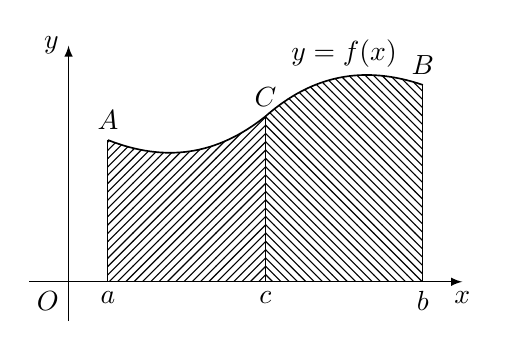
\begin{tikzpicture}[>=latex,scale=1.0]
  \draw[->](-0.5,0)--(5,0)node[below]{$x$};
  \draw[->](0,-0.5)--(0,3.0)node[left]{$y$};
  \node at (0,0)[below left]{$O$};
  \draw[semithick](0.5,1.8)node[above]{$A$}to[bend right](2.5,2.1)node[above]{$C$}to[bend left](4.5,2.5)node[above]{$B$};
  \draw(0.5,1.8)--(0.5,0)node[below]{$a$};
  \draw(2.5,2.1)--(2.5,0)node[below]{$c$};
  \draw(4.5,2.5)--(4.5,0)node[below]{$b$};
  \fill[pattern=north east lines](0.5,0)--(0.5,1.8)to[bend right](2.5,2.1)--(2.5,0);
  \fill[pattern=north west lines](2.5,0)--(2.5,2.1)to[bend left](4.5,2.5)--(4.5,0);
  \node at (3.5,2.9){$y=f(x)$};
\end{tikzpicture}
\end{document}